\subsection{Excercise APIDIagramAMRentalManagementV1.0}
TODO Add introduction
The API diagram of \texttt{AM-RentalManagementV1.0} is shown in \autoref{fig:ad_am-rental_management_v1.0}.
\subsubsection*{Derivation of the API Diagram}
An API diagram models the relevant entities depending on the type of API, in this case, \hfill \linebreak \texttt{RentalManagementV1.0} is an application microservice.
In an AM API diagram, relations between the application entities and the entities from other API diagrams occur.
A copy of the API diagram can be found on \url{https://gitlab.kit.edu/kit/cm/teaching/carrentalapp/0.doccarrentalappv1/-/blob/main/figures/ad_am-rental_management_v1.0.png?ref_type=heads} is shown in \autoref*{fig:ad_am-rental_management_v1.0}.

% Which artifacts are used to derive the API diagram
Since \texttt{RentalManagementV1.0} interacts with the \texttt{DM-CarV1.0} domain microservice, the DM API diagram is one artifact used to derive the AM API diagram.
Using the DM API diagram, the application entity \texttt{Car} is modeled.
Next, the entity diagram of \texttt{CarRental} is used to derive the application entities, their functions and their relations.
This entity diagram is shown in \autoref{fig:extendedEntityDiagram}
Yet, not all functions can be derived by \texttt{CarRental} alone.
The Use Cases of \texttt{CarRental} are used to derive functions too.
Advancing in this thesis, these Use Cases are also used to derive the CLI commands for \texttt{CarRentalCLI}.
Despite not all commands being implemented in this microservice, the functions for renting and canceling a rental are implemented, being specified by the Use Cases and the according CLI commands.

% How are the entities and methods established
The application entities \texttt{Customer} and \texttt{Rental} are derived from the entity diagram \autoref{fig:extendedEntityDiagram}.
Both entities keep the same attributes and relations as in the entity diagram.
The entity \texttt{Car} is derived from the DM API diagram, yet the relation between \texttt{Car} and \texttt{Rental} stays the same as in the entity diagram.
Last, the collection \texttt{Rentals} is newly created.
It contains a list of rentals and the \texttt{listAvailableCars} function returning a list of available cars.
Therefore, it is derived from the general structure and functionality of \texttt{DM-CarV1.0}'s \texttt{Cars} collection.

\begin{figure}
    \centering
    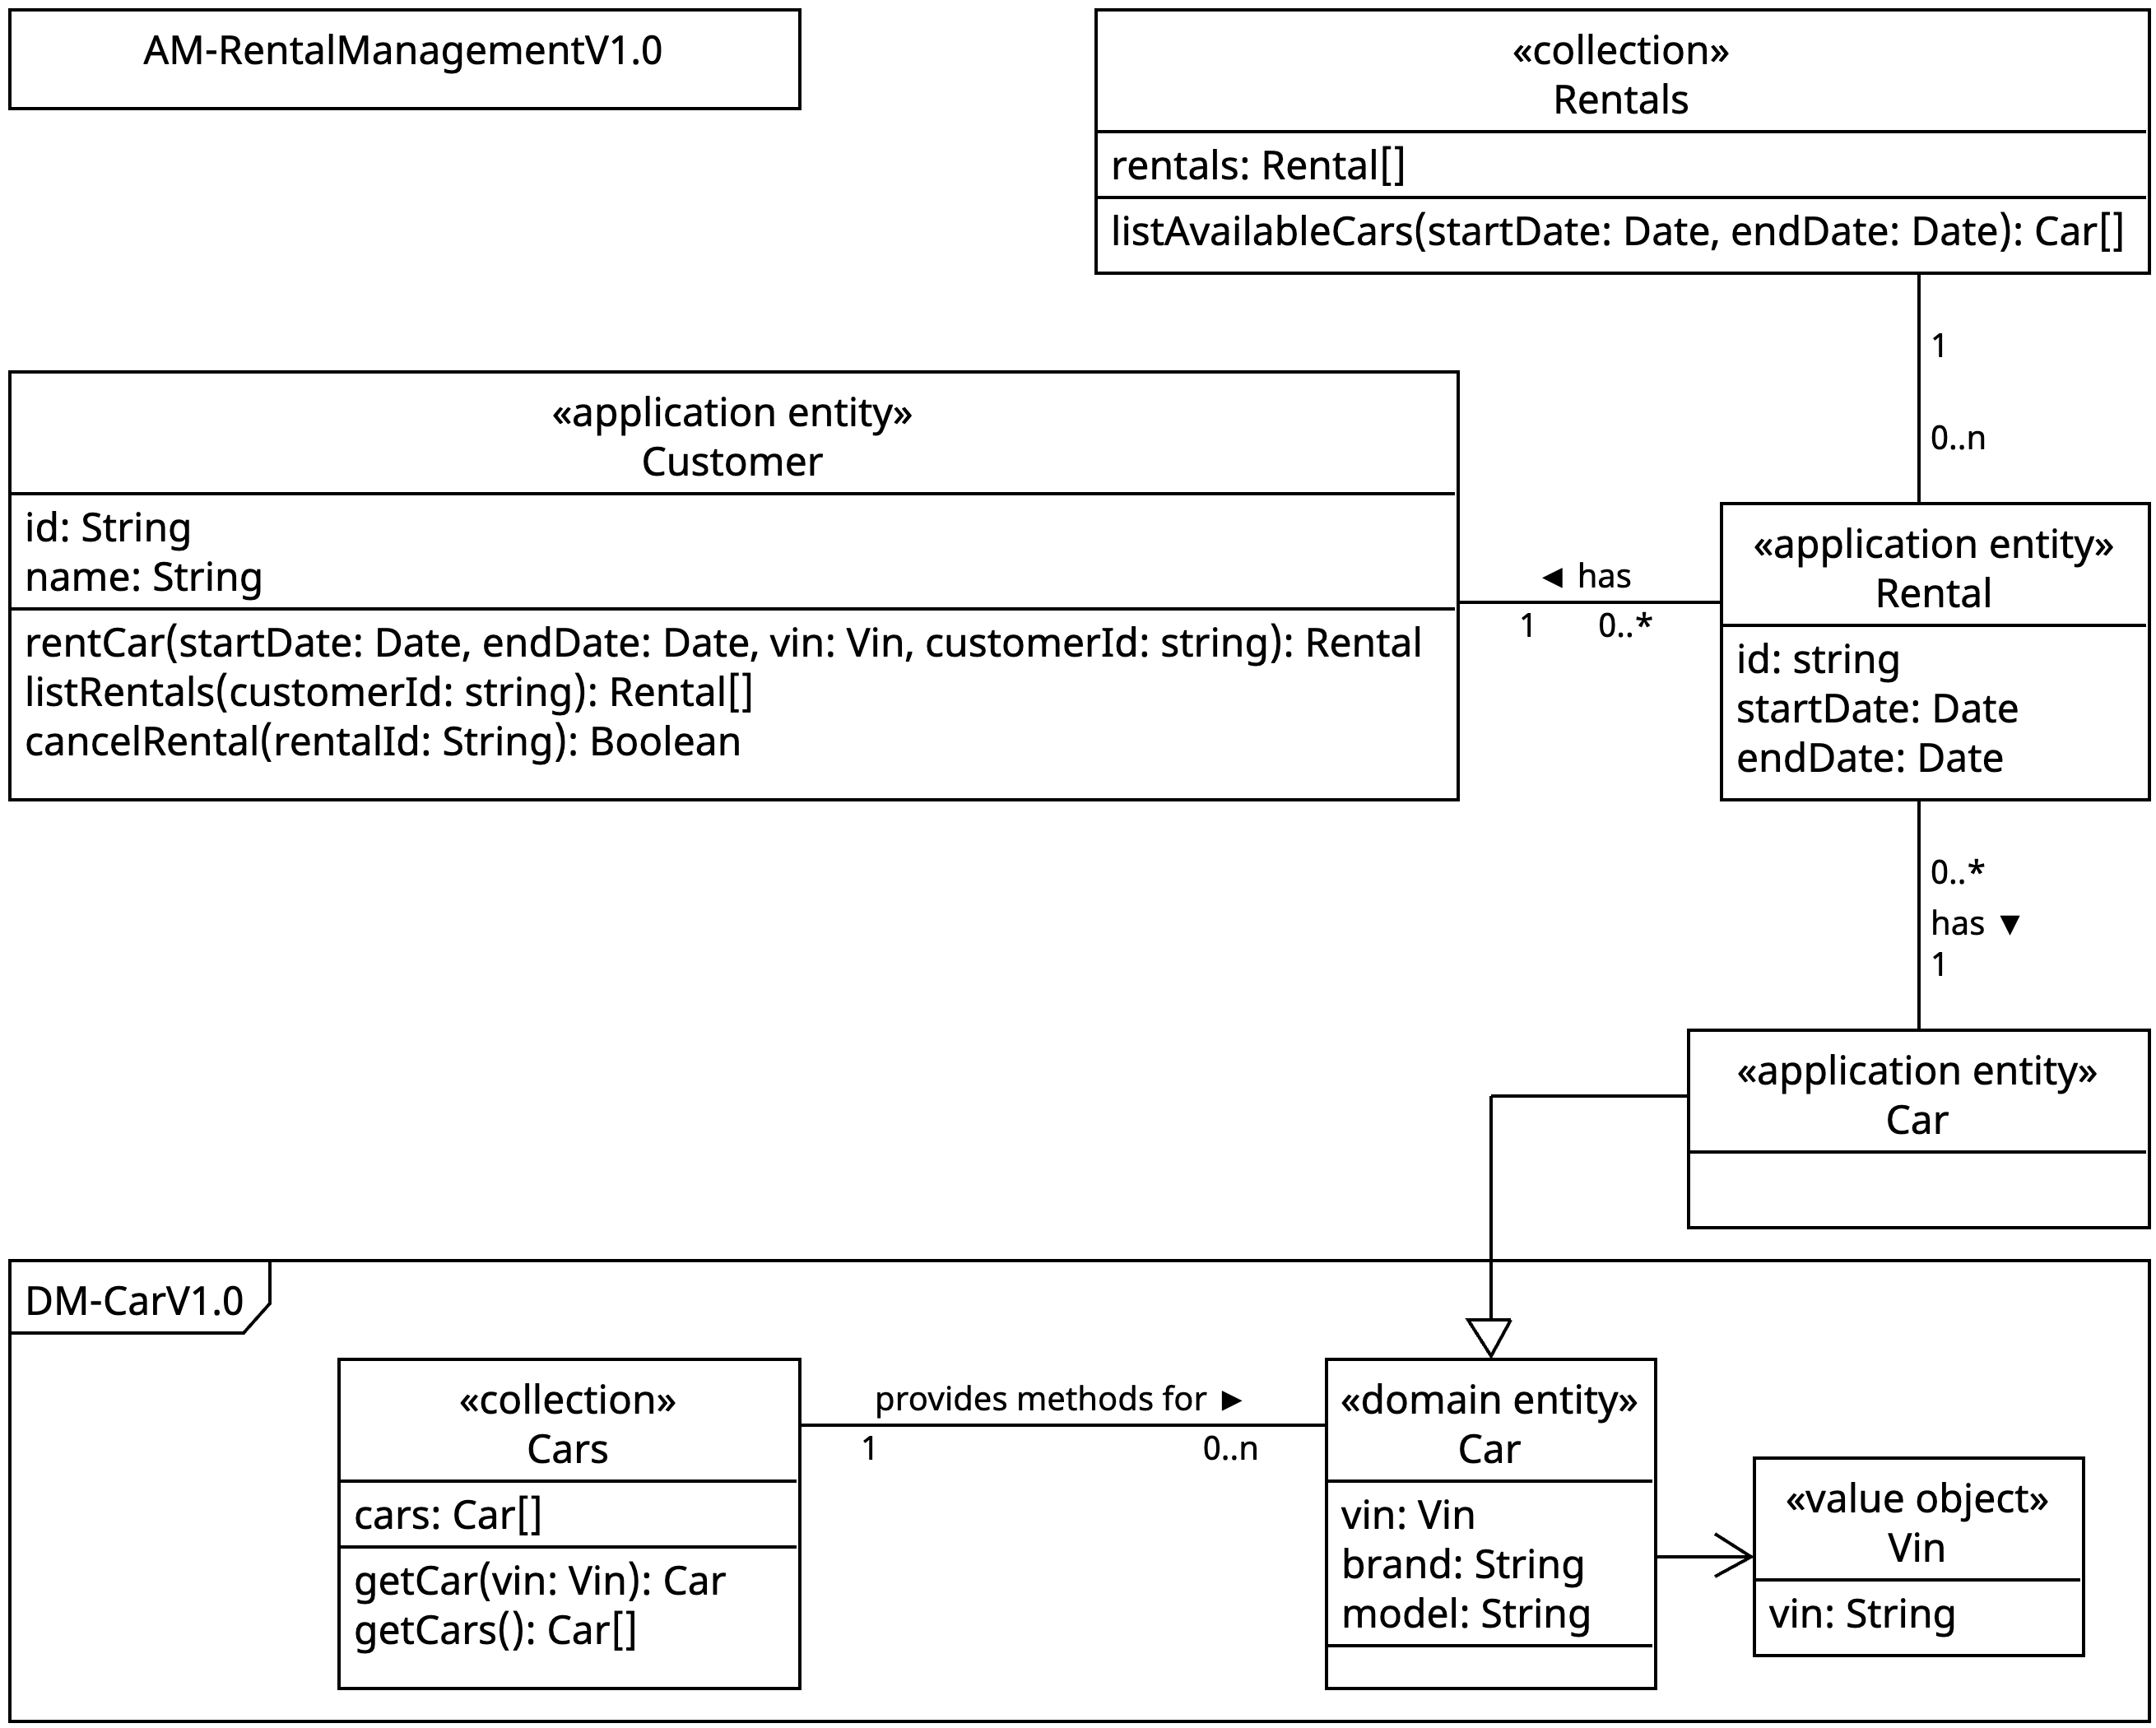
\includegraphics[width=0.8\textwidth]{figures/microservices/rentalManagement/ms_rentalManagement_apiDiagram.png}
    \caption{API Diagram of \texttt{AM-RentalManagementV1.0}}
    \label{fig:ad_am-rental_management_v1.0}
\end{figure}

\subsubsection*{Versioning of the API Diagram}
The version numbers are created using C\&M's versioning as specified in \cite{CM-G-Ver}.
% Explanation of the versioning concept for API diagrams
The initial version of an AM-API diagram is \texttt{1.0}.
The version of an AM API is specified for the first time when the diagram is initially created and reviewed.
It is important to keep the same version for specification and implementation.
The version number is increased when changes occur in the AM-API diagram.
% Explain version numbers of AM-RM and the included DM-Car
Since \texttt{RentalManagementV1.0} and \texttt{DM-CarV1.0} are the initial versions of each microservice, both chosen versions are \texttt{1.0}.

% Which part (X.Y) of the version number is increased when a method RegisterCustomer() is added => what's the new version number
This task assumes a version number to be structured as \texttt{(X.Y)}.
According to the mentioned versioning concept, \texttt{Y} changes when a new function is added to the AM-API diagram.
Therefore, after adding the function \texttt{RegisterCustomer} to the AM-API diagram, the version number is \texttt{1.1}.

\subsubsection*{Relationship between Rental and Car}
% Explain the relationship and type
% Does it prevent different customers from renting the same car at the same time?
The \texttt{Rental} to \texttt{Car} relation is a many-to-one relation.
Therefore, each \texttt{Rental} can only be assigned to exactly one \texttt{Car}.
Yet, a \texttt{Car} can be assigned to multiple \texttt{Rentals}.
The cars can be the same or different, which means that multiple rentals can exist for the same \texttt{Car}.
Due to no function checking if the \texttt{Car} is already rented, it is possible to create overlapping rentals for the same \texttt{Car}.

% If not, how can this be prevented?
There are some possibilities to prevent overlapping rentals.
One possibility is to check if the \texttt{Car} is already rented when renting a \texttt{Car}.
This could be done in the \texttt{rentCar} function of the \texttt{customer} application entity.
Another possibility is to work with the collection \texttt{Rentals} instead of working with the \texttt{Rental} application entity.
This way, the collection can check whether the \texttt{Car} is already rented for the given timeslot.

\subsubsection*{Relation of Entities Car}
% Describe the relation between application entity and domain entity car
This relation is a so-called inheritance relation.
This means, that the application entity \texttt{Car} inherits the attributes and functions from the domain entity \texttt{Car} and extends it with additional, application-related functions and attributes if necessary.
Since the domain entity \texttt{Car} gets its attributes and methods from the collection \texttt{Cars} and the value object \texttt{Vin}, the application entity \texttt{Car} also inherits parts of \texttt{Cars} and the value object \texttt{Vin}.
Thus, the application entity \texttt{Car} is an application-specific specialization of the domain entity \texttt{Car}.

% How do they relate
Both microservices relate in their attributes.
Since the application entity \texttt{Car} inherits from the domain entity \texttt{Car}, they both share the same attributes.

% What are the differences
They differ in their context and therefore their usage.
The domain entity \texttt{Car} is used in the domain microservice \texttt{DM-CarV1.0} which is responsible for CRUD operations provided by the collection \texttt{Cars}.
The application entity \texttt{Car} is used in the application microservice \texttt{AM-RentalManagementV1.0} which is responsible for renting and canceling rentals.
Therefore the application entity will be used in the context of a rental, while the domain entity will be used in the context of the CRUD operations.

\subsubsection*{API Style}
This lecture introduces two API styles: gRPC and ReST.
% Which API style is more appropriate
As mentioned in \autoref{subsec:rest_and_grpc} gRPC and ReST are two different approaches to implementing an API.
Their main difference is their orientation in the way they communicate.
While gRPC is method-oriented, ReST is resource-oriented.
Therefore the API operations of gRPC are methods, while the API operations of ReST are resources.
ReST helps to build a distributed system that handles clearly defined and identifiable resources.

\texttt{AM-RentalManagementV1.0} is a microservice that is responsible for managing, therefore creating and canceling, rentals.
This implies a function-oriented approach, due to the focus on managing instead of providing resources.
A more performant and efficient way of communication will be preferred over a more resource-oriented approach.
Therefore, gRPC is the more appropriate API style for \texttt{AM-RentalManagementV1.0}.